\section {Complexidade do problema da bissecção}
	Nesta seção veremos duas reduções que provam que o problema 
	da bissecção mínima é NP-Completo~(NP-Difícil 
	por não ser um problema de decisão),
	usando o fato de
	que a versão de decisão do
	problema {\sc max2sat} é NP-completa.

	Primeiramente, vamos definir alguns problemas para facilitar
	a compreensão das reduções.

	\medskip

	\begin{prob}[{\sc max2sat}($C,k$) -- Satisfatibilidade máxima com no máximo 
	dois literais por cláusula{~\cite{GareyJS76}}]
		Dado um conjunto~$C$ com~$p$ cláusulas distintas na forma 
		disjuntiva, com no máximo
		dois literais cada, e um inteiro~$k\le p$,
		decidir se existem valores para cada uma das variáveis, de forma
		que~$k$ ou mais cláusulas sejam verdadeiras.

		%~$C_i=(x_1 x_2)$,
	\end{prob}

	\medskip

	\begin{prob}[MaxCut($G,W$) -- Corte Máximo]
		Dado um grafo~${G}$
		%onde cada uma das arestas tem peso 1, 
		e um inteiro positivo~${W}$, decidir se existe um
		corte~$(T,F)$ em $G$ tal 
		que~${e_G(T,F)\ge W}$.
		
	\end{prob}

	

	% \begin{prob}[Corte mínimo em subconjuntos de mesmo tamanho 
	% {~\cite{GareyJS76}}]
	% 	Dado um grafo~$G(V,E)$, onde cada uma das arestas tem 
	% 	peso 1, e um inteiro positivo~$W\le|E|$, encontrar um
	% 	conjunto de vértices~$S\subseteq V$ tal 
	% 	que~$e_G(S,V\setminus~S)\ge W$.
		
	% \end{prob}

	\bigskip
	\bigskip
	\bigskip

	\subsection{Redução do \textbf{\textsc {max2sat}} para MaxCut}

		Dada uma instância~$(C,k)$ do problema {\sc max2sat}, 
		precisamos construir uma instância~$(G,W)$
		do problema MaxCut usando a resução que será descrita abaixo.
		Para isso vamos definir alguns conceitos referentes
		ao problema {\sc max2sat}:
		\begin{itemize}
			\item $p = $ número de cláusulas em~$C$
			\item $n = $ número de variáveis distintas em~$C$
		\end{itemize}

		% A redução consiste em criar um grafo~${G=(V,E)}$, de 
		% acordo com uma entrada para o problema {\sc max2sat}.
		% Segue o conjunto de vértices e arestas de~$G$, 
		% respectivamente.
		
		\begin{align}
			V = \ &\{x_i: 1\le i\le n\} \ \cup \nonumber\\
				&\{\overline{x_i}: 1\le i\le n\} \ \cup\nonumber\\ 
				&\{T_j: 0\le j\le 3p\} \ \cup \nonumber\\
				&\{F_j: 0\le j\le 3p\} \ \cup \nonumber\\
				&\{t_{ij}: 1\le i\le n, 0\le j\le 3p\} 
					\ \cup \nonumber\\
				&\{f_{ij}: 1\le i\le n, 0\le j\le 3p\}\nonumber
		\end{align}

		\begin{align}
			E_1= \ &\{ \{T_i,F_j\}: 0\le i\le 3p, 0\le j\le 3p\}\ \cup 
					\nonumber\\
				&\{\{t_{ij}, f_{ij}\}: 1\le i\le n, 
					0\le j\le 3p\}\ \cup \nonumber \\
				&\{\{x_i, f_{ij}\}: 1\le i\le n, 
					0\le j\le 3p\} \ \cup \nonumber \\
				&\{\{\overline{x_i}, t_{ij}\}: 1\le 
					i\le n, 0\le j\le 3p\} \nonumber
		\end{align}

		% \begin{align}
		% 	E_1=&\textcolor{blue}{\{ \{T_i,F_j\}: 0\le i\le 
		% 		3p, 0\le j\le 3p\}} &\cup \nonumber\\
		% 		&\textcolor{green!70}{\{\{t_{ij}, f_{ij}\}: 1\le i\le n, 
		% 			0\le j\le 3p\}} &\cup \nonumber \\
		% 		&\textcolor{brown}{\{\{x_i, f_{ij}\}: 1\le i\le n, 
		% 			0\le j\le 3p\}} &\cup \nonumber \\
		% 		&\textcolor{violet}{\{\{\overline{x_i}, t_{ij}\}: 1\le 
		% 			i\le n, 0\le j\le 3p\}} \nonumber \\
		% \end{align}

		E para cada uma das~$p$ cláusulas da forma~$C_i=(a_i\lor b_i)$, 
		temos também as arestas a seguir.

		\begin{align}
			E_2= \ &\{ \{a_i,b_i\}: 1\le i\le p, a_i\ne b_i \}\ \cup 
					\nonumber\\
				&\{\{a_i, F_{2\cdot i-1}\}: 1\le i\le p\}\ \cup \nonumber \\
				&\{\{b_i, F_{2\cdot i}\}: 1\le i\le p\} \nonumber
		\end{align}

		Dessa forma, temos o grafo~${G = (V,E)}$, com~${E=E_1\cup E_2}$.
		Segue abaixo um exemplo de como ficaria~$G$ sendo gerado por
		uma cláusula do tipo~${(x_1\lor \overline{x_2})}$.
		As arestas de~$E_2$ estão representadas pela cor 
		\textcolor{red}{\textbf {vermelha}}.

		\bigskip
		\bigskip

		\begin{center} 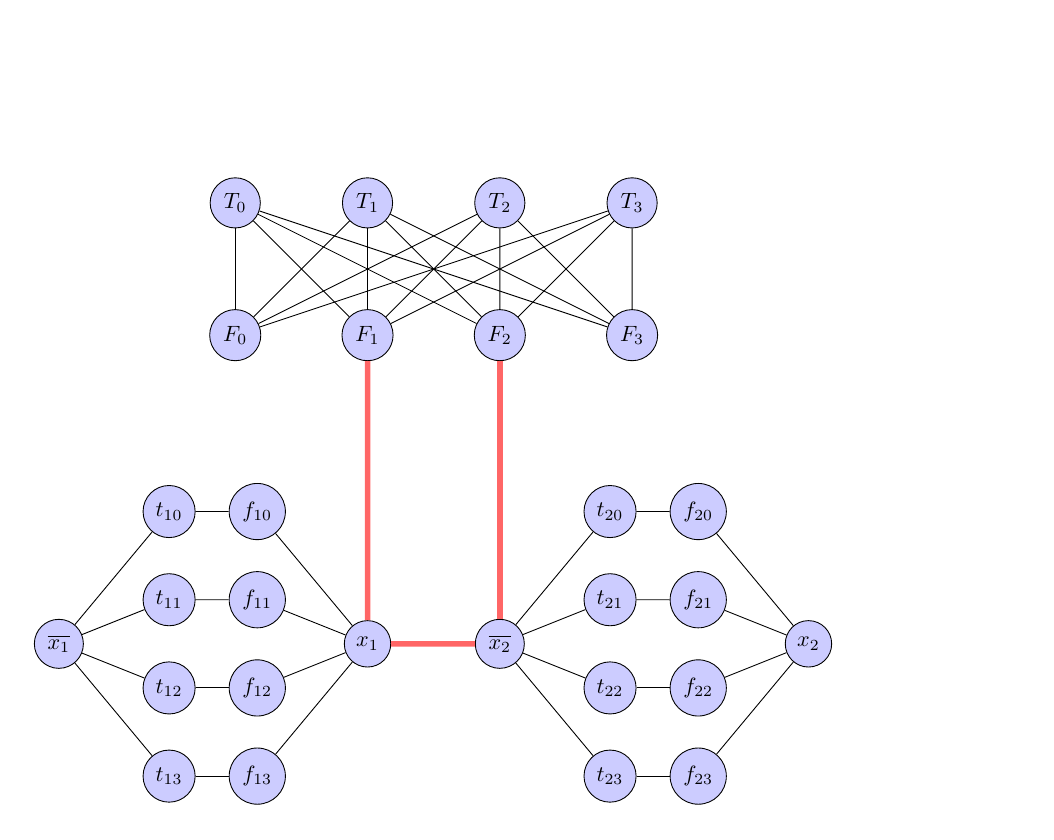
\begin{tikzpicture}
			[scale=.7,auto=left,every node/.style={circle, 
			draw=black,
			fill=blue!20}]
		\scalebox{0.8}{
			\node (t0) at (4, 13)  {$T_0$};
			\node (t1) at (7, 13)  {$T_1$};
			\node (t2) at (10,13)  {$T_2$};
			\node (t3) at (13,13)  {$T_3$};

			\node (f0) at (4, 10)  {$F_0$};
			\node (f1) at (7, 10)  {$F_1$};
			\node (f2) at (10,10)  {$F_2$};
			\node (f3) at (13,10)  {$F_3$};




			\node (t10) at (2.5,6)  {$t_{10}$};
			\node (t11) at (2.5,4)  {$t_{11}$};
			\node (t12) at (2.5,2)  {$t_{12}$};
			\node (t13) at (2.5,0)  {$t_{13}$};	

			\node (f10) at (4.5,6)  {$f_{10}$};
			\node (f11) at (4.5,4)  {$f_{11}$};
			\node (f12) at (4.5,2)  {$f_{12}$};
			\node (f13) at (4.5,0)  {$f_{13}$};
			  
			\node (f20) at (14.5,6)  {$f_{20}$};
			\node (f21) at (14.5,4)  {$f_{21}$};
			\node (f22) at (14.5,2)  {$f_{22}$};
			\node (f23) at (14.5,0)  {$f_{23}$};

			\node (t20) at (12.5,6)  {$t_{20}$};
			\node (t21) at (12.5,4)  {$t_{21}$};
			\node (t22) at (12.5,2)  {$t_{22}$};
			\node (t23) at (12.5,0)  {$t_{23}$};

			
			


			\node (x1n) at (0,3)  {$\overline{x_1}$};
			\node (x1)  at (7,3)  {$x_1$};
			\node (x2n)  at (10,3)  {$\overline{x_2}$};
			\node (x2) at (17,3)  {$x_2$};


			\foreach \from/\to in {t0/f0,t0/f1,t0/f2,t0/f3,
			t1/f0,t1/f1,t1/f2,t1/f3,
			t3/f0,t3/f1,t3/f2,t3/f3,
			t2/f0,t2/f1,t2/f2,t2/f3}%%%%
			\draw[] (\from) -- (\to);

			\foreach \from/\to in {t10/f10,t11/f11,t12/f12,t13/f13,
			t20/f20,t21/f21,t22/f22,t23/f23}%%%%
			\draw[] (\from) -- (\to);

			\foreach \from/\to in {t10/x1n,t11/x1n,t12/x1n,t13/x1n,
			t20/x2n,t21/x2n,t22/x2n,t23/x2n}
			\draw[] (\from) -- (\to);

			\foreach \from/\to in {x1/f10,x1/f11,x1/f12,x1/f13,
			x2/f20,x2/f21,x2/f22,x2/f23}
			\draw[] (\from) -- (\to);

			\foreach \from/\to in {x1/x2n,x1/f1,x2n/f2}
			\draw[draw=red!60, line width=2.5pt] (\from) -- (\to);
		}
		\end{tikzpicture} \end{center}

		\bigskip
		\bigskip

		Se encontrarmos um corte~$(T,F)$ em~$G$ tal 
		que~${e_G(T, F)\ge |A_1| + 2\cdot k}$, 
		então teremos que, para todo vértice do tipo~$x_i$,
		se~${x_i\in T}$, a variável que ele representa será
		verdadeira, já se~${x_i\in F}$, a variável que ele representa
		será falsa. Tendo que as variáveis possuem os valores conforme
		o que foi dito anteriormente, $k$ ou mais cláusulas serão 
		verdadeiras.

		\bigskip
		\bigskip
		\bigskip
		\bigskip
		\bigskip

		\begin{teo}
			A instância~$(G,W)$ de MaxCut tem solução se e somente se
			a instância~$(C,k)$ de {\sc max2sat} tem solução.
		\end{teo}

		\begin{proof}
		Mostraremos agora que para todas as entradas do problema
		{\sc max2sat}, existe uma solução da sua redução para o problema
		MaxCut.
		Para isso, vamos supor que já temos um conjunto de valores
		para as variáveis do problema {\sc max2sat} de forma que~$k$ ou mais
		cláusulas sejam verdadeiras.

		Sabemos que existem no máximo~$2p$ arestas do 
		tipo~${\{x_i,F_j\}}$ ou ${\{\overline{x_i},F_j\}}$. Dado 
		que~${2p<3p+1}$,
		que as funções~${f(i)=2\cdot i - 1}$ e~${g(i)=2\cdot i}$ têm 
		imagem ímpar e par, respectivamente, e ambas são injetoras, 
		portanto, temos que cada~$F_i$ se liga a apenas um vértice
		do tipo~$x_i$ ou~${\overline{x_i}}$.

		Definiremos agora os vértices contidos nos 
		subconjuntos~$T$ e~$F$ de~$G$.
		Suponhamos que para todo~${i\in[0,3p]}$,~${T_i\in T}$ 
		e~${F_i\in F}$ e
		para todo~${j\in[1,n]}$ e ${k\in[0,3p]}$, ~$x_j$ pertence ao 
		mesmo subconjunto que~$t_{jk}$ e ambos não pertencem ao mesmo 
		subconjunto que~$\overline{x_j}$ e que~$f_{jk}$.
		Assim sendo, temos que todas as arestas de~$E_1$ estão no 
		corte~$(T,F)$.
		Suponhamos também que se a variável~$x_i$ é verdadeira,
		então, o vértice~$x_i$ está em $T$, e se mantermos as 
		propriedades que foram citadas anteriormente, isso não afetará o 
		fato de todas as arestas de~$E_1$ estarem no corte~$(T,F)$.
		Portanto, assumiremos inicialmente que essa é a disposição dos 
		vértices nos subconjuntos~$T$ e~$F$.

		Temos que, em uma cláusula~${C_i=(a_i,b_i)}$, ou
		apenas um dos literais é satisfeito, ambos são ou nenhum
		deles é.
		\begin{enumerate}
			\item Se apenas um dos literais é satisfeito, temos que,
			das arestas formadas pela cláusula~$C_i$, duas
			estão no corte~$(T,F)$ e uma está fora.
			\item Se os dois literais são satisfeitos, também teremos
			duas arestas no corte~$(T,F)$ e uma fora.
			\item Já no caso de nenhum literal ser satisfeito, nenhuma
			dessas arestas da cláusula estará no corte~$(T,F)$.
		\end{enumerate}

		Podemos ver isso de forma mais clara na imagem a seguir.

		\begin{center} 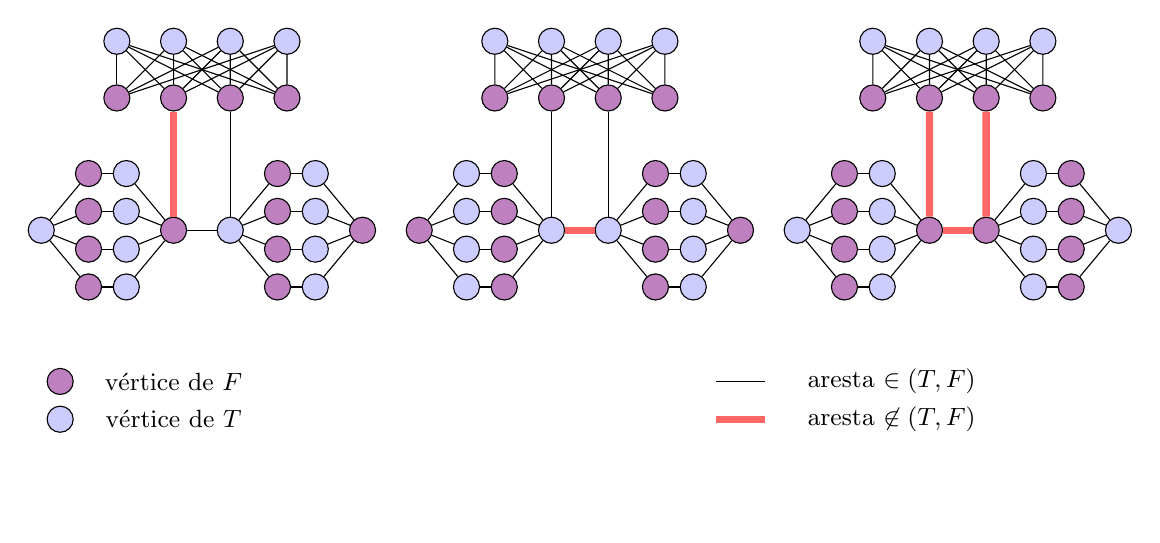
\begin{tikzpicture}
			[scale=.24,auto=left,every node/.style={circle, 
			draw=black,
			fill=blue!20}]
			


			\node (t0_) at (4 +20,13)  {};
			\node (t1_) at (7 +20,13)  {};
			\node (t2_) at (10+20,13)  {};
			\node (t3_) at (13+20,13)  {};

			\node [fill=violet!50](f0_) at (4 +20,10)  {};
			\node [fill=violet!50](f1_) at (7 +20,10)  {};
			\node [fill=violet!50](f2_) at (10+20,10)  {};
			\node [fill=violet!50](f3_) at (13+20,10)  {};

			\node (t10_) at (2.5+20,6)  {};
			\node (t11_) at (2.5+20,4)  {};
			\node (t12_) at (2.5+20,2)  {};
			\node (t13_) at (2.5+20,0)  {};	

			\node [fill=violet!50](f10_) at (4.5+20,6)  {};
			\node [fill=violet!50](f11_) at (4.5+20,4)  {};
			\node [fill=violet!50](f12_) at (4.5+20,2)  {};
			\node [fill=violet!50](f13_) at (4.5+20,0)  {};
			  
			\node (f20_) at (14.5+20,6)  {};
			\node (f21_) at (14.5+20,4)  {};
			\node (f22_) at (14.5+20,2)  {};
			\node (f23_) at (14.5+20,0)  {};

			\node [fill=violet!50](t20_) at (12.5+20,6)  {};
			\node [fill=violet!50](t21_) at (12.5+20,4)  {};
			\node [fill=violet!50](t22_) at (12.5+20,2)  {};
			\node [fill=violet!50](t23_) at (12.5+20,0)  {};
			
			\node [fill=violet!50](x1n_) at (0 +20, 3)  {};
			\node (x1_)  at (7 +20, 3)  {};
			\node (x2n_) at (10+20, 3) {};
			\node [fill=violet!50](x2_)  at (17+20, 3) {};






			\node (t0__) at (4 +40,13)  {};
			\node (t1__) at (7 +40,13)  {};
			\node (t2__) at (10+40,13)  {};
			\node (t3__) at (13+40,13)  {};

			\node [fill=violet!50](f0__) at (4 +40,10)  {};
			\node [fill=violet!50](f1__) at (7 +40,10)  {};
			\node [fill=violet!50](f2__) at (10+40,10)  {};
			\node [fill=violet!50](f3__) at (13+40,10)  {};

			\node [fill=violet!50](t10__) at (2.5+40,6)  {};
			\node [fill=violet!50](t11__) at (2.5+40,4)  {};
			\node [fill=violet!50](t12__) at (2.5+40,2)  {};
			\node [fill=violet!50](t13__) at (2.5+40,0)  {};	

			\node (f10__) at (4.5+40,6)  {};
			\node (f11__) at (4.5+40,4)  {};
			\node (f12__) at (4.5+40,2)  {};
			\node (f13__) at (4.5+40,0)  {};
			  
			\node [fill=violet!50](f20__) at (14.5+40,6)  {};
			\node [fill=violet!50](f21__) at (14.5+40,4)  {};
			\node [fill=violet!50](f22__) at (14.5+40,2)  {};
			\node [fill=violet!50](f23__) at (14.5+40,0)  {};

			\node (t20__) at (12.5+40,6)  {};
			\node (t21__) at (12.5+40,4)  {};
			\node (t22__) at (12.5+40,2)  {};
			\node (t23__) at (12.5+40,0)  {};
			
			\node (x1n__) at (0 +40, 3)  {};
			\node [fill=violet!50](x1__)  at (7 +40, 3)  {};
			\node [fill=violet!50](x2n__) at (10+40, 3) {};
			\node (x2__)  at (17+40, 3) {};






			\node (t0) at (4 ,13)  {};
			\node (t1) at (7 ,13)  {};
			\node (t2) at (10,13)  {};
			\node (t3) at (13,13)  {};

			\node [fill=violet!50](f0) at (4 ,10)  {};
			\node [fill=violet!50](f1) at (7 ,10)  {};
			\node [fill=violet!50](f2) at (10,10)  {};
			\node [fill=violet!50](f3) at (13,10)  {};



			\node [fill=violet!50](t10) at (2.5,6)  {};
			\node [fill=violet!50](t11) at (2.5,4)  {};
			\node [fill=violet!50](t12) at (2.5,2)  {};
			\node [fill=violet!50](t13) at (2.5,0)  {};	

			\node (f10) at (4.5,6)  {};
			\node (f11) at (4.5,4)  {};
			\node (f12) at (4.5,2)  {};
			\node (f13) at (4.5,0)  {};
			  
			\node (f20) at (14.5,6)  {};
			\node (f21) at (14.5,4)  {};
			\node (f22) at (14.5,2)  {};
			\node (f23) at (14.5,0)  {};

			\node [fill=violet!50](t20) at (12.5,6)  {};
			\node [fill=violet!50](t21) at (12.5,4)  {};
			\node [fill=violet!50](t22) at (12.5,2)  {};
			\node [fill=violet!50](t23) at (12.5,0)  {};


			\node (x1n) at (0,3)  {};
			\node [fill=violet!50](x1)  at (7,3)  {};
			\node (x2n) at (10,3) {};
			\node [fill=violet!50](x2)  at (17,3) {};



			\node (l1) at (1,-7)  {};
			\node [fill=violet!50](l2)  at (1,-5)  {};
			\node [draw=none, fill=none] at 
				(7,-5) {\small{vértice de $F$}};
			\node [draw=none, fill=none] at 
				(7,-7) {\small{vértice de $T$}};
			\node [draw=none, fill=none](a1) at (35,-5) {};
			\node [draw=none, fill=none](a1_) at (39,-5) {};
			\node [draw=none, fill=none](a2) at (35,-7) {};
			\node [draw=none, fill=none](a2_) at (39,-7) {};
			\node [draw=none, fill=none] at 
				(45,-5) {\small{aresta $\in(T,F)$}};
			\node [draw=none, fill=none] at 
				(45,-7) {\small{aresta $\not\in(T,F)$}};
			\foreach \from/\to in {t0_/f0_,t0_/f1_,t0_/f2_,t0_/f3_,
			t1_/f0_,t1_/f1_,t1_/f2_,t1_/f3_,
			t3_/f0_,t3_/f1_,t3_/f2_,t3_/f3_,
			t2_/f0_,t2_/f1_,t2_/f2_,t2_/f3_}%%%%
			\draw[] (\from) -- (\to);

			\foreach \from/\to in 
			{t10_/f10_,t11_/f11_,t12_/f12_,t13_/f13_,
			t20_/f20_,t21_/f21_,t22_/f22_,t23_/f23_}%%%%
			\draw[] (\from) -- (\to);

			\foreach \from/\to in 
			{t10_/x1n_,t11_/x1n_,t12_/x1n_,t13_/x1n_,
			t20_/x2n_,t21_/x2n_,t22_/x2n_,t23_/x2n_}
			\draw[] (\from) -- (\to);

			\foreach \from/\to in 
			{x1_/f10_,x1_/f11_,x1_/f12_,x1_/f13_,
			x2_/f20_,x2_/f21_,x2_/f22_,x2_/f23_,x1_/f1_,x2n_/f2_}
			\draw[] (\from) -- (\to);

			\foreach \from/\to in {x1_/x2n_}
			\draw[draw=red!60, line width=2.7pt] (\from) -- (\to);


			

			\foreach \from/\to in {t0__/f0__,t0__/f1__,t0__/f2__,t0__/f3__,
			t1__/f0__,t1__/f1__,t1__/f2__,t1__/f3__,
			t3__/f0__,t3__/f1__,t3__/f2__,t3__/f3__,
			t2__/f0__,t2__/f1__,t2__/f2__,t2__/f3__}%%%%
			\draw[] (\from) -- (\to);

			\foreach \from/\to in 
			{t10__/f10__,t11__/f11__,t12__/f12__,t13__/f13__,
			t20__/f20__,t21__/f21__,t22__/f22__,t23__/f23__}%%%%
			\draw[] (\from) -- (\to);

			\foreach \from/\to in 
			{t10__/x1n__,t11__/x1n__,t12__/x1n__,t13__/x1n__,
			t20__/x2n__,t21__/x2n__,t22__/x2n__,t23__/x2n__}
			\draw[] (\from) -- (\to);

			\foreach \from/\to in 
			{x1__/f10__,x1__/f11__,x1__/f12__,x1__/f13__,
			x2__/f20__,x2__/f21__,x2__/f22__,x2__/f23__,a1/a1_}
			\draw[] (\from) -- (\to);

			\foreach \from/\to in {x1__/x2n__,x1__/f1__,x2n__/f2__,a2/a2_}
			\draw[draw=red!60, line width=2.7pt] (\from) -- (\to);




			\foreach \from/\to in {t0/f0,t0/f1,t0/f2,t0/f3,
			t1/f0,t1/f1,t1/f2,t1/f3,
			t3/f0,t3/f1,t3/f2,t3/f3,
			t2/f0,t2/f1,t2/f2,t2/f3}%%%%
			\draw[] (\from) -- (\to);

			\foreach \from/\to in {t10/f10,t11/f11,t12/f12,t13/f13,
			t20/f20,t21/f21,t22/f22,t23/f23}%%%%
			\draw[] (\from) -- (\to);

			\foreach \from/\to in {t10/x1n,t11/x1n,t12/x1n,t13/x1n,
			t20/x2n,t21/x2n,t22/x2n,t23/x2n}
			\draw[] (\from) -- (\to);

			\foreach \from/\to in {x1/f10,x1/f11,x1/f12,x1/f13,
			x2/f20,x2/f21,x2/f22,x2/f23,x2n/f2,x1/x2n}
			\draw[] (\from) -- (\to);

			\foreach \from/\to in {x1/f1}
			\draw[draw=red!60, line width=2.7pt] (\from) -- (\to);
		\end{tikzpicture} \end{center}

		Sabe-se que temos~$2k$ ou mais arestas de~$E_1$ que estão no
		corte~$(T,F)$, pois, para cada uma das~$k$ cláusulas
		verdadeiras, teremos duas arestas de~$E_1$ no corte, como
		o mostrado anteriormente.

		Se houvesse alguma aresta duplicada (duas arestas que ligam
		os mesmos vértices), teríamos um problema na contagem de
		arestas dentro e fora do corte.
		Isso poderia ocorrer no caso de duas cláusulas serem 
		idênticas,~${C_i=C_j=(a_i,b_i)}$.
		Isso faria com que houvesse uma aresta duplicada entre
		os vértices~$a_1$ e~$b_i$, mas isso não acontece, dado que
		no enunciado é assumido que as cláusulas são distintas.
		Também não há o problema de dois vértices estarem em cláusulas
		diferentes, dado que para cada cláusula, os vértices se ligam
		a um~$F_i$ diferente.
		E mesmo se repetirmos as variáveis na mesma cláusula, cada
		elemento da cláusula se ligará a um~$F_i$ diferente.

		\bigskip

		Mostramos que existe uma solução, em MaxCut, 
		para todas as entradas do
		problema {\sc max2sat} reduzidas para MaxCut, de forma que
		a solução do MaxCut leva a uma solução de {\sc max2sat}.
		Agora mostraremos que qualquer solução obtida em 
		uma redução para MaxCut levará a uma solução de {\sc max2sat}.
	\end{proof}

\subsection{Redução MaxCut para Bissecção}

% \begin{center} \begin{tikzpicture}
% 	[scale=.7,auto=left,every node/.style={circle, 
% 	draw=black,
% 	fill=blue!20}]

% 	\node (an1) at (-3 -7, 1) {$v_1$};
% 	\node (an2) at (-5 -7, 2) {$v_2$};
% 	\node (an3) at (-3 -7, 10) {$v_3$};
% 	\node (an4) at (-5 -7, 9) {$v_4$};
% 	\node (an5) at (-6 -7, 6) {$v_5$};

% 	%legenda
% 	\node [draw=none, fill=none](a1)  at (-5  ,-0.5) {};
% 	\node [draw=none, fill=none](a1_) at (-6.4,-0.5) {};
% 	\node [draw=none, fill=none](a2)  at (-5  ,-1.5) {};
% 	\node [draw=none, fill=none](a2_) at (-6.4,-1.5) {};

% 	\node [draw=none, fill=none] at 
% 		(-3,-0.5) {\small{aresta $\in(T,F)$}};
% 	\node [draw=none, fill=none] at 
% 		(-3,-1.5) {\small{aresta $\not\in(T,F)$}};
	

% 	\foreach \from/\to in {an1/an2,an1/an3,an1/an4,an2/an4,an2/an5,
% 	a1/a1_}
% 	\draw[draw=red!60, line width=2.7pt] (\from) -- (\to);

% 	\foreach \from/\to in {an1/an5,an2/an3,an3/an4,an3/an5,an4/an5,
% 	a2/a2_}
% 	\draw[draw=CornflowerBlue,line width=1.3pt] (\from) -- (\to);

% \end{tikzpicture} \end{center}


\begin{center} 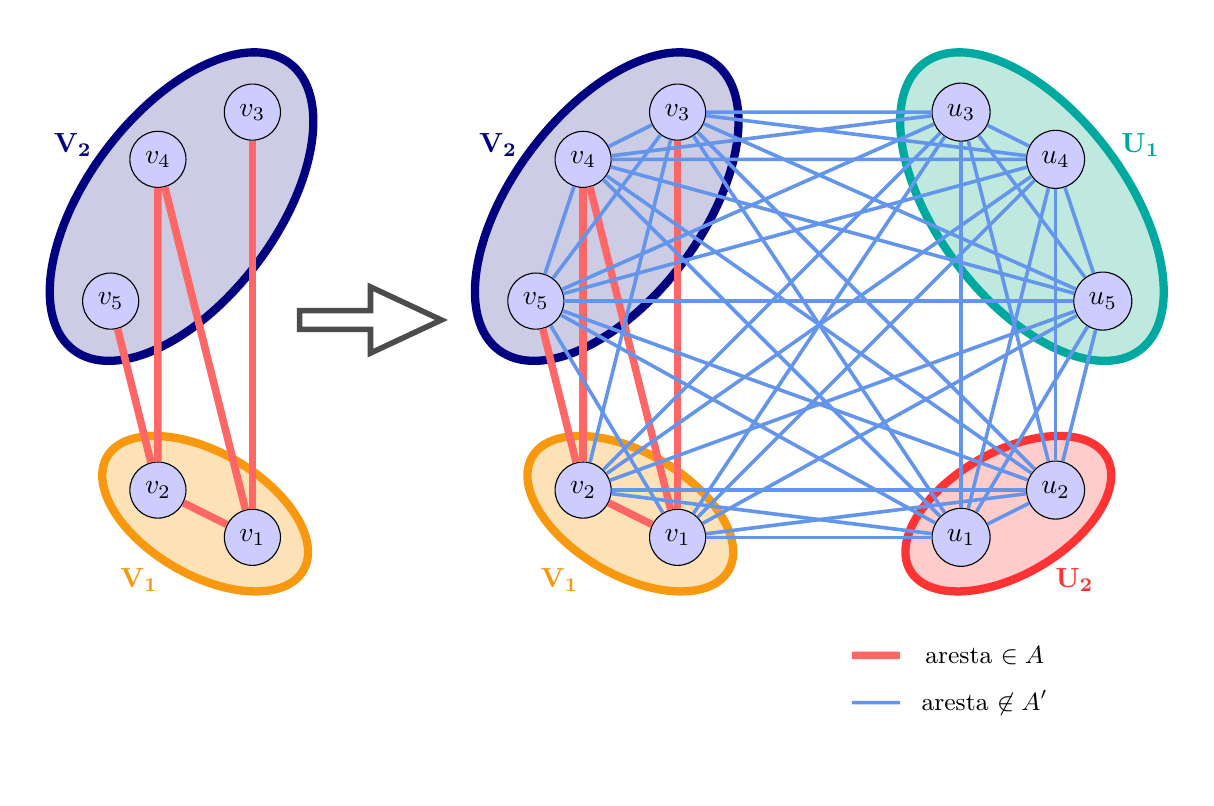
\begin{tikzpicture}
	[scale=.6,auto=left,every node/.style={circle, 
	draw=black,
	fill=blue!20}]

	\draw [rotate around={60:(-13,1.5)}, draw=YellowOrange, fill=YellowOrange!25,line width=3pt] (-13,1.5) 
		ellipse (1.3cm and 2.4cm);
	\draw [rotate around={143:(-13.5,8)}, draw=NavyBlue, fill=NavyBlue!20,line width=3pt] (-13.5,8) 
		ellipse (2cm and 3.8cm);
	



	\draw [rotate around={60:(-4,1.5)}, draw=YellowOrange, fill=YellowOrange!25,line width=3pt] (-4,1.5) 
		ellipse (1.3cm and 2.4cm);
	\draw [rotate around={143:(-4.5,8)}, draw=NavyBlue, fill=NavyBlue!20,line width=3pt] (-4.5,8) 
		ellipse (2cm and 3.8cm);




	\draw [rotate around={-60:(4,1.5)}, draw=red!80, fill=red!20,line width=3pt] (4,1.5) 
		ellipse (1.3cm and 2.4cm);
	\draw [rotate around={-143:(4.5,8)}, draw=Emerald, fill=Emerald!25,line width=3pt] (4.5,8) 
		ellipse (2cm and 3.8cm);
	

	\node [text=YellowOrange,draw=none, fill=none] at (-14.4,0.1){$\mathbf{V_1}$};
	\node [text=NavyBlue,draw=none, fill=none] at (-15.8,9.3){$\mathbf{V_2}$};

	\node [text=YellowOrange,draw=none, fill=none] at (-5.5,0.1){$\mathbf{V_1}$};
	\node [text=NavyBlue,draw=none, fill=none] at (-6.8,9.3){$\mathbf{V_2}$};


	\node [text=red!80,draw=none, fill=none] at (5.4,0.1){$\mathbf{U_2}$};
	\node [text=Emerald,draw=none, fill=none] at (6.8,9.3){$\mathbf{U_1}$};

	\node (an1) at (-12, 1) {$v_1$};
	\node (an2) at (-14, 2) {$v_2$};
	\node (an3) at (-12, 10) {$v_3$};
	\node (an4) at (-14, 9) {$v_4$};
	\node (an5) at (-15, 6) {$v_5$};

	\node (v1) at (-3, 1)  {$v_1$};
	\node (v2) at (-5, 2)  {$v_2$};
	\node (v3) at (-3, 10) {$v_3$};
	\node (v4) at (-5, 9)  {$v_4$};
	\node (v5) at (-6, 6)  {$v_5$};

	\node (u1) at (3, 1)  {$u_1$};
	\node (u2) at (5, 2)  {$u_2$};
	\node (u3) at (3, 10) {$u_3$};
	\node (u4) at (5, 9)  {$u_4$};
	\node (u5) at (6, 6)  {$u_5$};

	%legenda
	\node [draw=none, fill=none](a1)  at (2  ,-1.5) {};
	\node [draw=none, fill=none](a1_) at (0.4,-1.5) {};
	\node [draw=none, fill=none](a2)  at (2  ,-2.5) {};
	\node [draw=none, fill=none](a2_) at (0.4,-2.5) {};

	\node [draw=none, fill=none] at 
		(3.5,-1.5) {\small{aresta $\in A$}};
	\node [draw=none, fill=none] at 
		(3.5,-2.5) {\small{aresta $\not\in A'$}};
	

	\foreach \from/\to in {v1/v4,v1/v2,v1/v3,v2/v4,v2/v5,
	a1/a1_,
	an1/an4,an1/an2,an1/an3,an2/an4,an2/an5}
	\draw[draw=red!60, line width=2.7pt] (\from) -- (\to);

	\foreach \from/\to in {v1/v5,v2/v3,v3/v4,v3/v5,v4/v5,
	u1/u2,u1/u3,u1/u4,u1/u5,u2/u3,u2/u4,u2/u5,u3/u4,u3/u5,u4/u5,
	v1/u1, v1/u2, v1/u3, v1/u4, v1/u5,
	v2/u1, v2/u2, v2/u3, v2/u4, v2/u5,
	v3/u1, v3/u2, v3/u3, v3/u4, v3/u5,
	v4/u1, v4/u2, v4/u3, v4/u4, v4/u5,
	v5/u1, v5/u2, v5/u3, v5/u4, v5/u5,
	a2/a2_}
	%an1/an5,an2/an3,an3/an4,an3/an5,an4/an5}
	\draw[draw=CornflowerBlue,line width=1.3pt] (\from) -- (\to);

	\draw [draw=black!70, line width=2pt]
		(-11. ,5.4) -- 
		(-11. ,5.8) --
		(-9.5 ,5.8) --
		(-9.5 ,6.3) --
		(-8.  ,5.6) --%%%
		(-9.5 ,4.9) --
		(-9.5 ,5.4) --
		cycle;

	

\end{tikzpicture} \end{center}
